\documentclass{article}
\usepackage[T1]{fontenc}
\usepackage[utf8]{inputenc}
\usepackage{graphicx}
\usepackage{float}

\usepackage{hyperref}
\urlstyle{same}

\title{Wielowarstwowy system rekrutacji dla szkół z interfejsem webowym i aplikacją mobilną - analiza techniczna rozwiązania}
\author{Andrzej Westfalewicz, Filip Zyskowski}
\date{7 listopada 2019}

\renewcommand*\contentsname{Spis treści}
\renewcommand\refname{Odwołania} 

% do wrapowania tekstu w tabelce
\usepackage{array}
\newcolumntype{L}{>{\centering\arraybackslash}m{10cm}}
% 
\usepackage{tabularx}

\begin{document}

\begin{titlepage}
\maketitle
\end{titlepage}

\tableofcontents

\pagebreak

\section{Architektura}
\subsection{Baza danych}
Jest odpowiedzialna za przechowywanie danych systemu. Znajdują się w niej główne obiekty systemu takie jak użytkownicy, kandydaci czy egzaminy. Z dostępnych systemów relacyjnych baz danych wybrany został MySQL Community Server, ponieważ jest popularnym i bezpłatnym rozwiązaniem.
\subsection{API}
Jest odpowiedzialne za dostęp do logiki biznesowej, zapis i odczyt danych, w szczególności zdjęć i dokumentów, przesłanych przez użytkowników. Umożliwia on pobranie przez przeglądarkę internetową Aplikacji webowej. Za pośrednictwem jego dokonywane są płatności przez bramkę płatniczą oraz wysyłane wiadomości e-mail. Do jego implementacji została wykorzystana technologia ASP.NET Core z uwagi na jej znajomość i popularność.
\subsection{Aplikacja webowa}
Umożliwia dostęp do systemu przez przeglądarkę internetową. Akcje użytkownika są interpretowane przez aplikację i wywołują odpowiednie akcje w API. Aby dane prezentowane na stronie były takie same na wszystkich urządzeniach, aplikacja nie przechowuje żadnych danych - są one pobierane z API. Zaimplementowana w popularnym frameworku Vue.js.
\subsection{Aplikacja mobilna}
Umożliwia dostęp do systemu przez telefon z systemem Android. Na tych urządzeniach nadal można się uzyskać dostęp do systemu poprzez mobilną przeglądarkę internetową, lecz aplikacja mobilna zapewnia znacznie większy komfort użytkowania na urządzeniach mobilnych. Akcje użytkownika są interpretowane przez aplikację i wywołują odpowiednie akcje w API. Zaimplementowana w frameworku NativeScript z nakładką umożliwiającą tworzenie aplikacji tak, jak w frameworku Vue.js.

\section{Wzorce projektowe modułów}
\subsection{Baza danych}
Baza została zaprojektowana zgodnie z podejściem \emph{code-first} z wykorzystaniem Entity Framework Core dla baz w systemie MySQL. Oznacza to tyle, że najpierw opisujemy schemat tabeli jako klasa w języku C\#, a potem jest ona mapowana na tabelę w bazie danych. Pozwala to również na modyfikowanie schematu bazy danych poprzez modyfikacje powyższych klas, za pomocą mechanizmu migracji dostarczonego przez Entity Framework. Pliki migracyjne reprezentujące historię zmian oraz ostateczny stan bazy danych są w katalogu Migrations wewnątrz projektu RecruitMe.Web.

\begin{figure}[H]
\centering
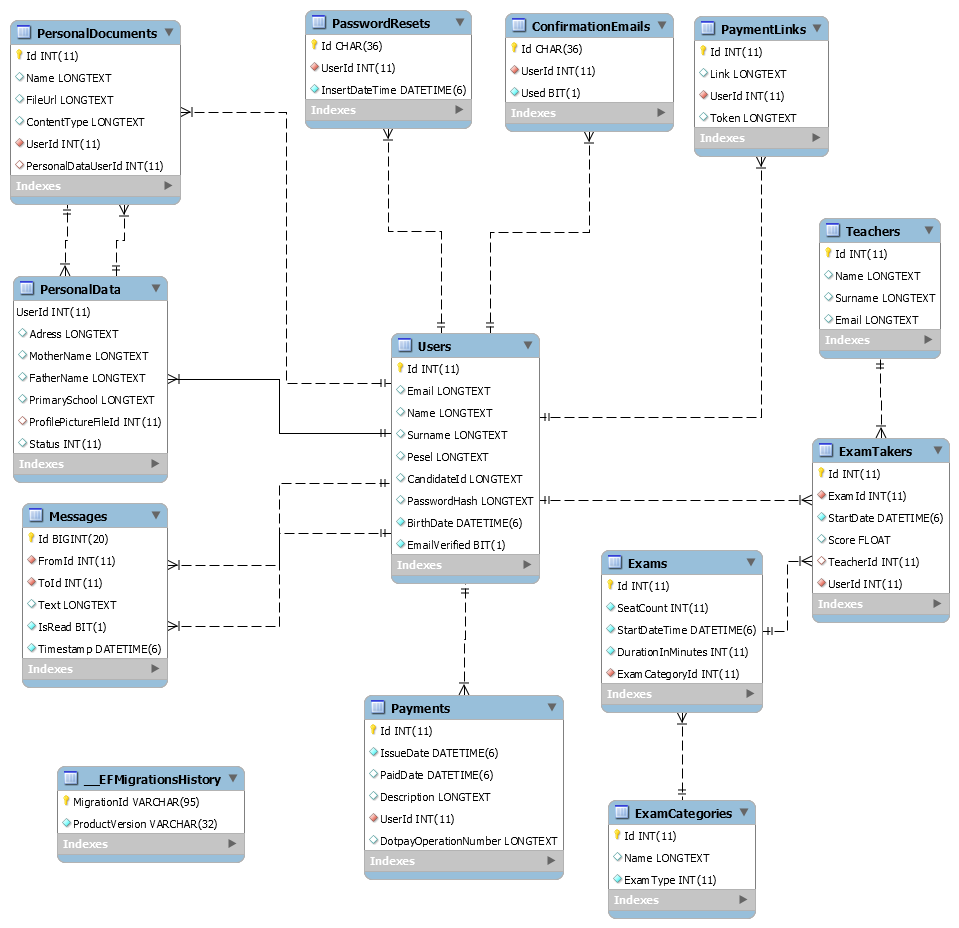
\includegraphics[scale=0.35]{images/model.png}
\caption{Obecny diagram schematu bazy}
\end{figure}

\subsection{Logika biznesowa}

\begin{itemize}
    \item Logika biznesowa została zorganizowana według reguły rozdzielenia komend i zapytań (Command Query Responsibility Segregation, CQRS). Zgodnie z nią akcje w systemie są podzielone na komendy - modyfikujące stan systemu i zwracające minimalną ilość danych (np. identifikatory) oraz zapytania, które zwracają dane. Stosując się do tej reguły system można lepiej optymalizować i taniej utrzymywać.
    \item Jeśli pomiędzy akcjami są jakieś zależności (jedna agreguje wiele innych lub działa na wyniku poprzedniej) zgodnie z wzorcem projektowym wstrzykiwania zależności (dependency injection, DI) akcje nie są tworzone wewnątrz klasy, lecz przekazywane do jej wnętrza przez konstruktor. Zastosowanie takiego wzorca umożliwia testowanie kodu.
    \item Część klas potrzebnych w warstwie logiki musi być zdefiniowana w warstwie API, dlatego stworzone zostały abstrakcyjne klasy i interfejsy, które są używane w miejscu gotowych klas w zgodzie z zasadą programowania do interfejsu (programming to interface). 
\end{itemize}
\subsection{API}
Zadaniem API jest pośredniczenie pomiędzy aplikacjami frontendowymi, a warstwą logiki. Aby nie zużywać transferu danych, część akcji jest agregowanych w jedną np.: zapis danych kandydata i zapytanie o nowe wartości. Metody kontrolerów wywoływane na żądania na dane endpointy definiują interfejs systemu - możliwe akcje użytkowników.\\
Dodatkowo API jest odpowiedzialne za autentykację użytkowników wykonujących żądania do systemu, czyli za tworzenie i walidację JWT, według standardu autentykacji OpenID Connect.
\subsection{Aplikacja webowa}
Aplikacja mobilna napisana została w frameworku JavaScriptowym Vue.js, który wymusza wzorzec MVVM. Warstwy odpowiadają za:
\begin{itemize}
    \item Model - żądania do API, 
    \item View - kod TypeScript,
    \item View-Model - kod html/css.
\end{itemize}
\subsection{Aplikacja mobilna}
Z racji, że aplikacja mobilna jest zaimplementowana w frameworku NativeScript z nakładką umożliwiającą pisanie aplikacji w Vue.js, został wykorzystany wzorzec MVVM.
\subsection{Testy}
Testują kluczowe elementy systemu (np. płatności).

\section{Komunikacja}
Komunikacja pomiędzy aplikacjami frontendowymi a API będzie się odbywała poprzez protokół HTTPS.
\\
Połączenie pomiędzy warstwy API a bazą danych będzie obsługiwane przez Entity Framework Core, który to obsługuje połączenia z bazami używając frameworka ADO.NET. Z kolei ADO.NET ustanawia połączenie poprzez sockety TCP/IP. 

\section{Opis modułów}
\subsection{Logika biznesowa}
Moduł logiki biznesowej znajduje się w projekcie RecruitMe.Logic. Został podzielony na części (domeny) według zadań, które dana część wykonuje. Implementacja każdej domeny jest umieszczona w osobnej przestrzeni nazw.

\subsubsection{RecruitMe.Logic.Data}
Zawiera abstrakcyjne klasy i interfejsy służące do przechowywania danych np. pośredniczący z bazą danych DbContext lub do przechowywania plików. W tej domenie znajdują się również klasy encji przechowywanych w bazie danych, które definiują jej schemat dołączony już wyżej.

\subsubsection{RecruitMe.Logic.Logging}
Zawiera klasy służące do logowania. Wybrana klasa jest wstrzykiwana do klas, które coś logują, aby ujednolicić proces zbierania logów.

\subsubsection{RecruitMe.Logic.Operations.Account}
Zawiera klasy implementujące proces rejestracji, logowania, sprawdzanie ID użytkownika itd. Proces rejestracji, przypomnienia loginu, resetu hasła opisują poniższe diagramy aktywności.
\begin{figure}[H]
\centering
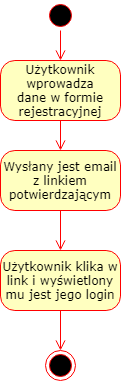
\includegraphics[scale=0.5]{images/Rejestracja.png}
\caption{Diagram aktywności procesu rejestracji}
\end{figure}

\begin{figure}[H]
\centering
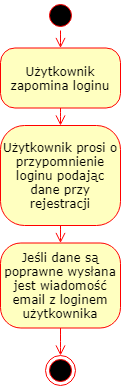
\includegraphics[scale=0.5]{images/przypomnienieloginu.png}
\caption{Diagram aktywności procesu przypomnienia loginu}
\end{figure}

\begin{figure}[H]
\centering
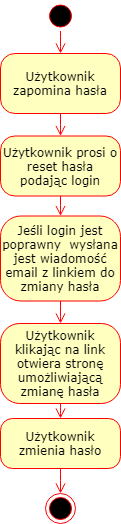
\includegraphics[scale=0.5]{images/resetHasla.png}
\caption{Diagram aktywności procesu resetu hasła}
\end{figure}

\subsubsection{RecruitMe.Logic.Operations.Email}
Zawiera klasy implementujące wysyłanie wiadomości email. Wysyłanie maili odbywa się za pomocą protokołu SMTP. Skrzynka, z której są wysyłane wiadomości może być podmieniona, jednak na czas rozwijania aplikacji został użyty adres "RecruitMeSystem@gmail.com".

\subsubsection{RecruitMe.Logic.Operations.Recruitment}
Zawiera klasy implementujące proces rekrutacji jak przesłanie danych, przesłanie dokumentów, zdjęcia lub rozmowy (chat) ze szkołą. Pliki będą przechowywane na dysku twardym poza bazą danych. Sposób zapisywania plików jest wstrzykiwany do domeny z projektu API.

\subsubsection{RecruitMe.Logic.Operations.Payments}
Zawiera klasy implementujące proces płatności. Klasy będą implementować operacje na bramce płatniczej DotPay. W bazie będą przechowywane tylko dane potrzebne do zweryfikowania, że na konto bankowe organizatora rekrutacji wpłynęły odpowiednie środki (to znaczy, że nie będziemy przechowywali takich danych jak numer karty kredytowej czy numeru CVV). \\
Proces wykonania transakcji, podobnie do procesu autentykacji OAuth, polega na przekierowaniu użytkownika na stronę DotPay z linkiem na który ma powrócić po dokonaniu transakcji oraz z zaszyfrowanymi informacjami.

\subsubsection{RecruitMe.Logic.Operations.Admin}
Zawiera klasy implementujące działania administratora, w szczególności edycję obiektów w bazie danych, generowanie i wczytywanie kart egzaminacyjnych.

\subsubsection{RecruitMe.Logic.Operations.Messages}
Zawiera klasy implementujące funkcjonalność chatu, dla kandydatów jak i dla administratora.

\subsection{Testy}
Do testów sprawdzających poprawność działania systemu i jego poszczególnych modułów zaliczamy testy jednostkowe oraz integracyjne. Każdy z testów zostanie przydzielony do odpowiedniej przestrzeni nazw względem domen, które testują.

\subsection{API}
Moduł API odpowiada za udostępnienie komunikacji pomiędzy modułem aplikacji webowej/mobilnej a modułem logiki biznesowej. Znajduje się on w folderze \emph{RecruitMe.Web/}. \\
Z aplikacji webowej/mobilnej wysyłane jest zapytanie na adres serwera systemu o jakieś dane. Moduł API przechwytuje to żądanie, sprawdza poprawność parametrów zapytania i, gdy spełnione są odpowiednie warunki (chociażby takie jak to, czy użytkownik jest zalogowany lub ma odpowiednie uprawnienia do wykonania danego zapytania), odsyła do aplikacji proszone dane lub informację, że jakaś czynność została wykonana pomyślnie. W przeciwnym wypadku moduł API zwraca aplikacji informację o nieudanym wykonaniu żądania wraz z odpowiednim kodem i informacją błędu.

\subsection{Aplikacja webowa}
Kod aplikacji webowej można znaleźć w folderze \emph{RecruitMe.WebApp/ClientApp/}. Ten folder jest podzielony na logiczne części, ułatwiające nawigację po module. Poza folderami znajdziemy plik \emph{boot.ts}, w którym zostało opisane mapowanie ścieżki adresu do odpowiedniego komponentu aplikacji oraz ogólna konfiguracja startowa aplikacji.
\subsubsection{Komponenty}
Folder \emph{components/} zawiera komponenty renderowane do widoków w aplikacji. Są one podzielone na foldery względem ścieżki, po jakiej się do nich można dostać (przykładowo: komponent do logowania znajdziemy w folderze \emph{components/account/login}). \\
Każdy komponent jest podzielony na dwa (lub trzy pliki): 
\begin{itemize}
    \item *.ts - model i logika komponentu
    \item *.vue.html - widok komponentu
    \item *.cs - stylowanie widoku (w większości zastąpione używając gotowych komponentów z paczki vuetify)
\end{itemize}
\subsubsection{Modele}
W folderze \emph{models/} znajdują się definicje modeli danych potrzebnych do wykonywania poprawnych zapytań do API oraz otrzymywania poprawnych odpowiedzi z API. \\
Każdy plik z o końcówce \emph{.model.ts} zawiera co najmniej interfejs, który specyfikuje format, w jakim powinniśmy wysłać zapytanie i otrzymać odpowiedź.
\subsubsection{Serwisy}
Folder \emph{services/} zawiera pliki o końcówce \emph{.service.ts}, które zawierają logikę łączenia się do API i zarządzania otrzymanymi z API danymi. Wykorzystywane są głównie w plikach \emph{*.ts} komponentów aplikacji.

\subsection{Aplikacja mobilna}
W głównym folderze projektu aplikacji mobilnej (Recruit.MobileApp/app/) mamy uporządkowaną strukturę plików i folderów odpowiadającą poszczególnym modułom zaimplementowanych w aplikacji mobilnej.

\subsubsection{ViewModele}
W folderze \emph{components/} są wszystkie viewmodele używane w aplikacji. Znajdziemy tam pliki z rozszerzeniem \emph{.vue}, które są rozmieszczone w odpowiednich podfolderach oznaczających w jakich operacjach będą się pojawiały poszczególne widoki (plik \emph{Login.vue} będzie znajdował się w podfolderze \emph{account/}, gdyż akcja logowania jest związana z operacjami na koncie użytkownika). \\
Pliki zawierają trzy główne sekcje rozdzielone znacznikami wymienionymi poniżej
\begin{itemize}
    \item \emph{<template>...</template>} - rozmieszczenie komponentów na ekranie telefonu
    \item \emph{<script>...</script>} - dane i logika modelu
    \item \emph{<style>...</style>} - wystylowanie komponentów
\end{itemize}

\subsubsection{Modele}
W folderze \emph{models/} znajdują się definicje modeli danych potrzebnych do wykonywania poprawnych zapytań do API oraz otrzymywania poprawnych odpowiedzi z API. \\
Każdy plik z rozszerzeniem \emph{.ts} zawiera co najmniej interfejs, który specyfikuje format, w jakim powinniśmy wysłać zapytanie i otrzymać odpowiedź.

\subsubsection{Serwisy}
Folder \emph{services/} zawiera pliki o rozszerzeniu \emph{.ts}, które zawierają logikę łączenia się do API i zarządzania otrzymanymi z API danymi. Niektóre pliki są pogrupowane w foldery, gdy pewne logiki należą do jednej kategorii (serwis użytkownika i serwis przechowywania danych logowania znajdą się w jednym folderze).

\subsubsection{Magazyn danych}
W folderze \emph{RecruitMe.MobileApp/} znajduje się plik o nazwie \emph{store.ts} będący wynikiem zastosowania biblioteki Vuex, który przechowuje dane pomiędzy widokami aplikacji. Obecnie jest wykorzystywany do utrzymywania tokenu zalogowanego użytkownika.

\section{Opis UI/UX}
\subsection{Aplikacja webowa}
Aplikacja webowa będzie korzystać z gotowych komponentów z biblioteki vuetify, które gwarantują przejrzysty i intuicyjne layout strony. Dodatkowo dzięki użyciu biblioteki bootstrap strona będzie responsywna, aby wyglądała dobrze na dużych jak i małych monitorach. W razie potrzeby niektóre elementy będą dopasowywane do stylu systemu za pomocą styli css.

\begin{figure}[H]
\centering
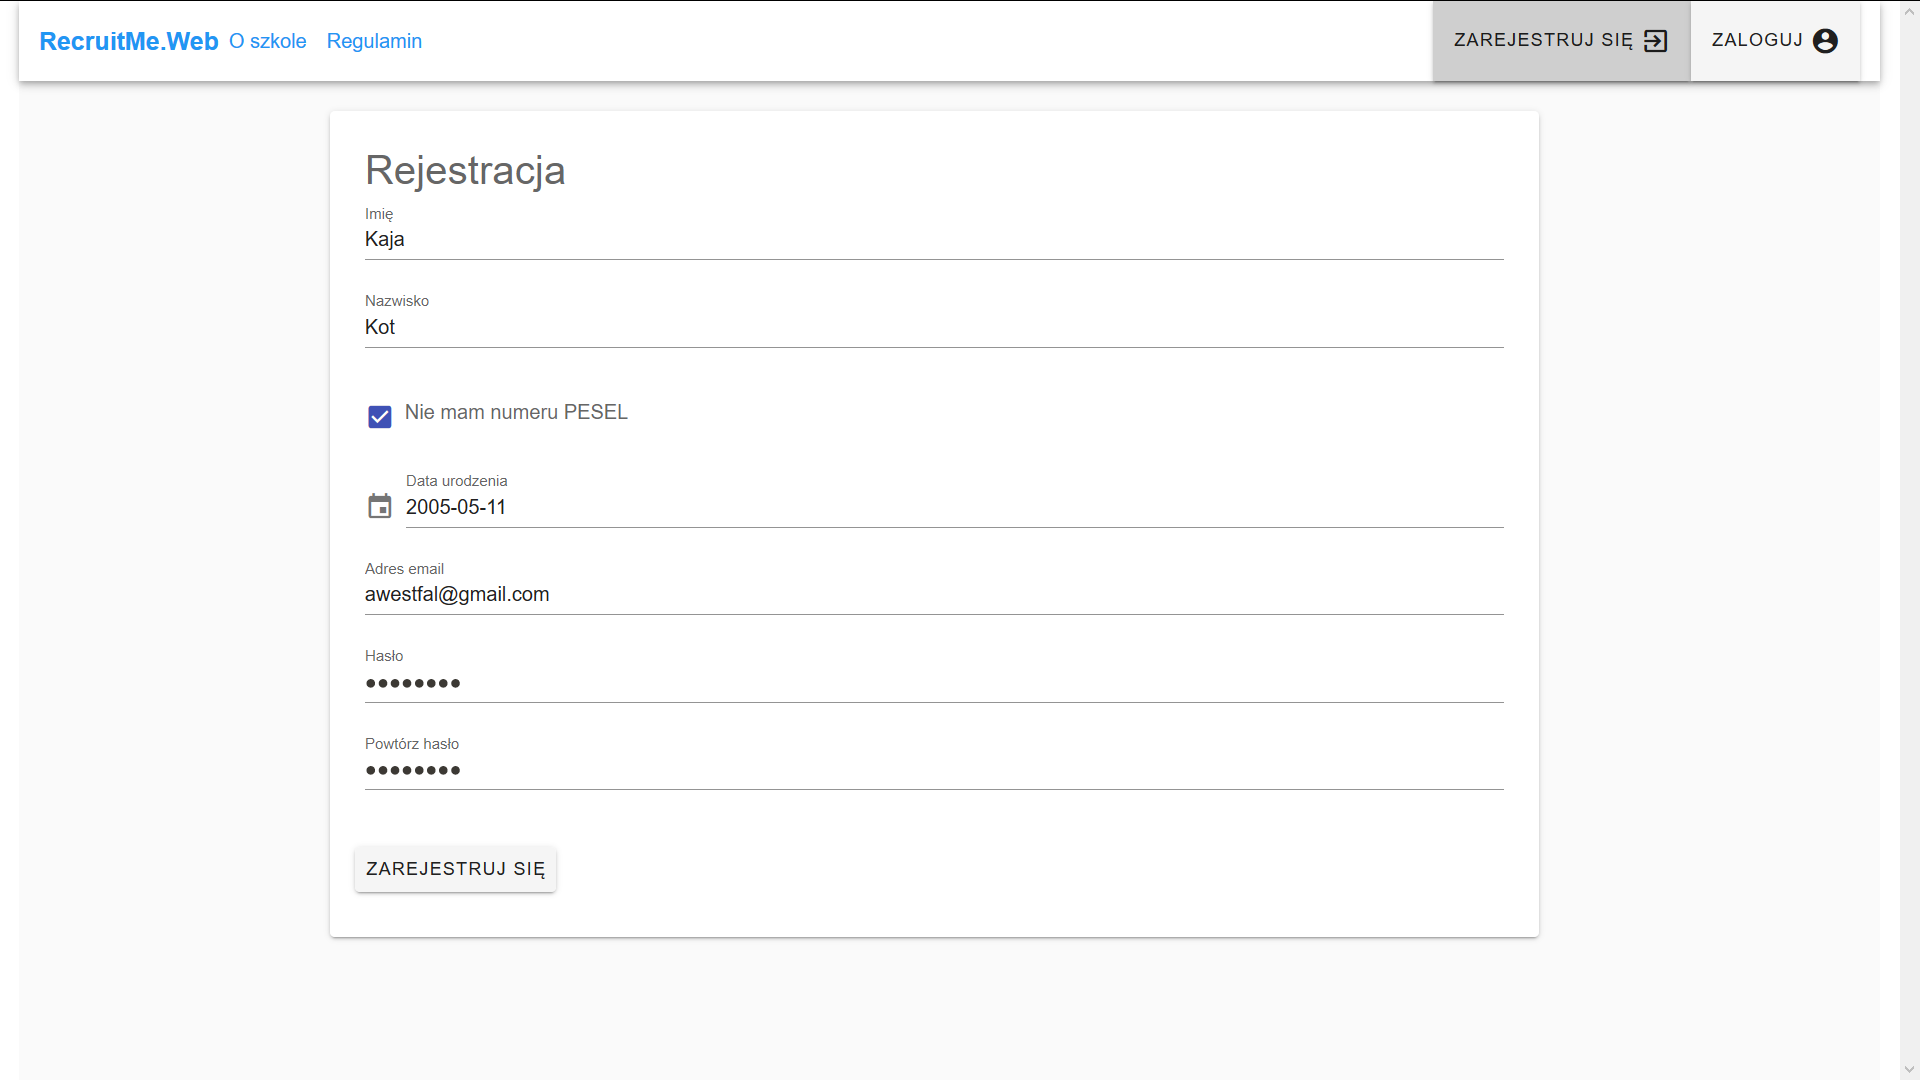
\includegraphics[scale=0.18]{images/rejestracjaMockup.png}
\caption{Przykładowy wygląd strony rejestracji}
\end{figure}

\begin{figure}[H]
\centering
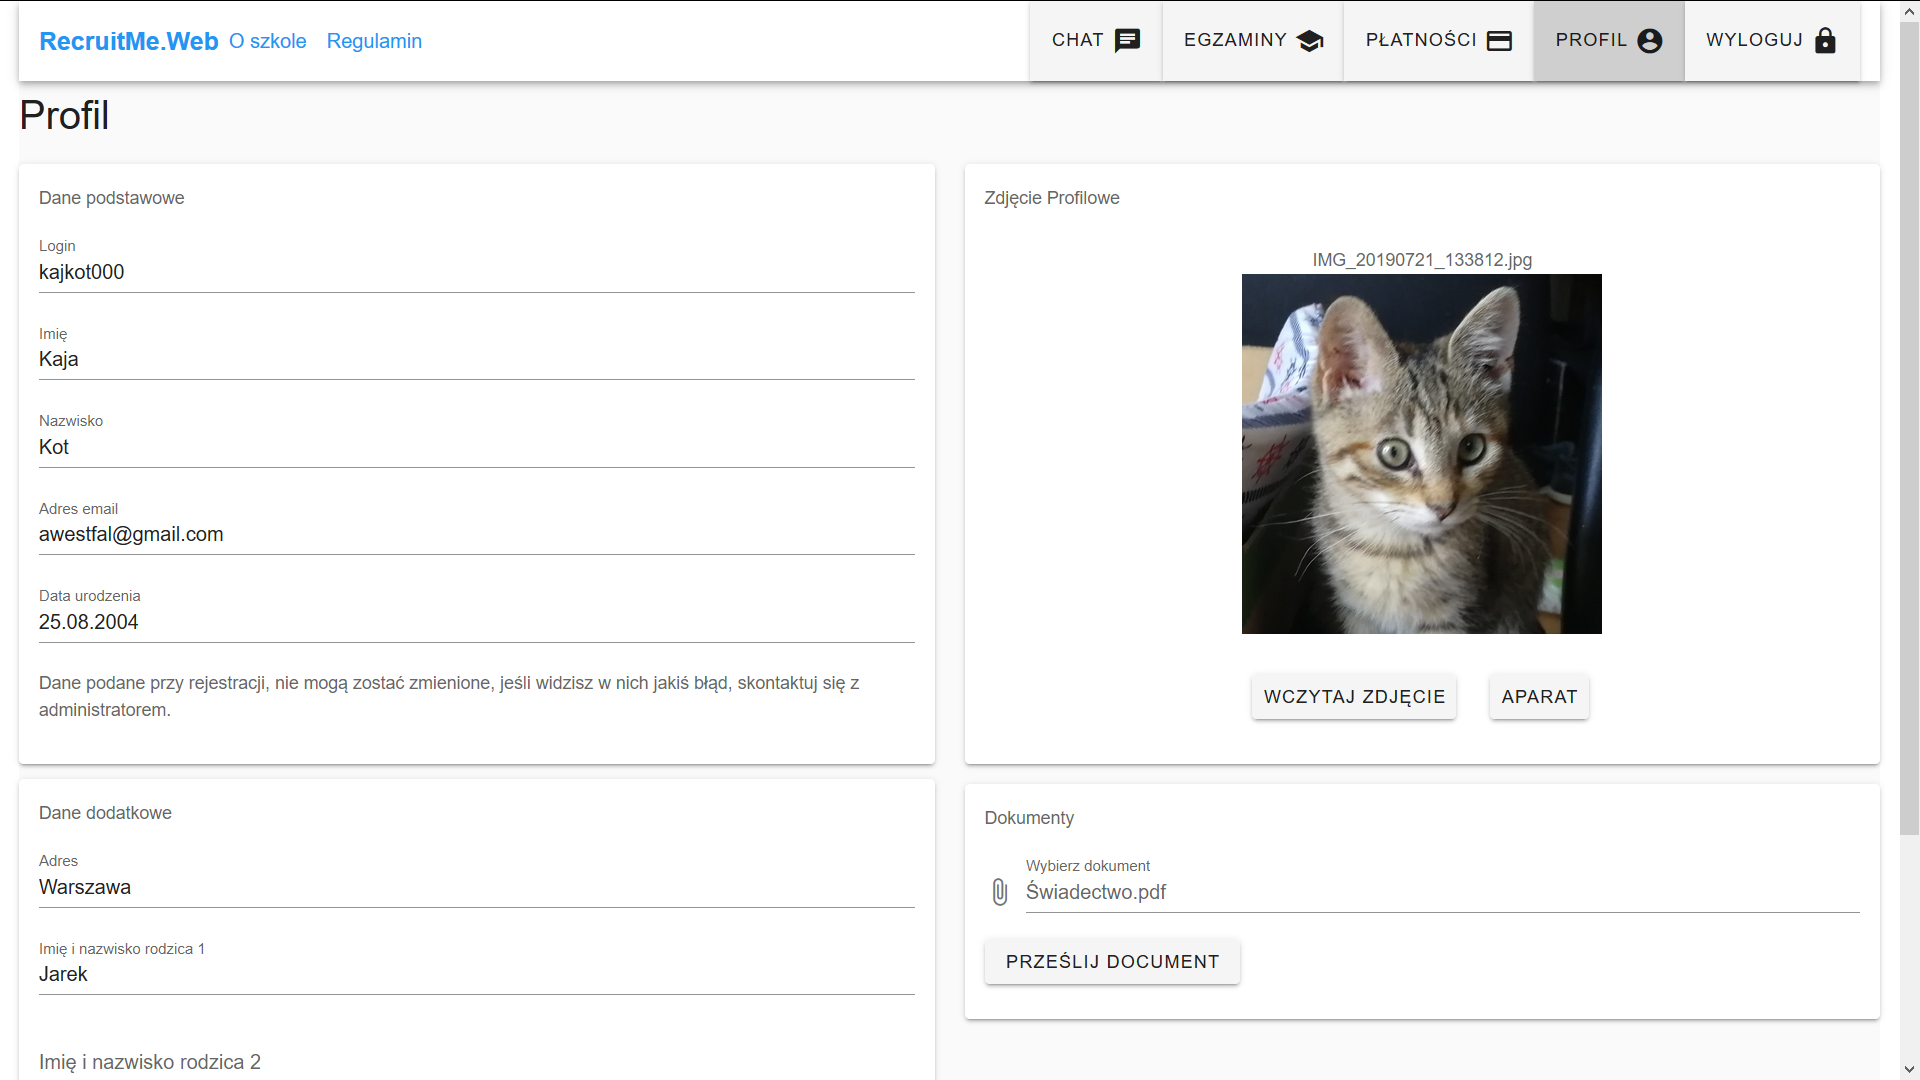
\includegraphics[scale=0.18]{images/profilMockup.png}
\caption{Przykładowy wygląd strony profilu kandydata}
\end{figure}


\subsection{Aplikacja mobilna}
Aplikacja mobilna z racji implementacji wybranego frameworka nie jest w stanie korzystać z tak szerokiej gamy komponentów i bibliotek co aplikacja webowa. Istnieje duże ograniczenie w dostosowywaniu kontrolek do własnej koncepcji spowodowane niezaimplementowaniem możliwości zmiany danego parametru zarówno przez twórców systemu Android jak i frameworka NativeScript. Z tego powodu, aplikacja mobilna będzie się posługiwała dużą ilością własnych stylów css oraz znaczącą liczbą małych bibliotek rozszerzających wygląd i funkcjonalność brakujących części widoku. \\

Aplikację mobilną można podzielić na dwie części - widoki przed zalogowaniem i po zalogowaniu. 
Na starcie, przed zalogowaniem użytkownik zobaczy duże logo aplikacji i pod spodem dwa przyciski prowadzące do ekranu logowania oraz ekranu rejestracji. W ekranie logowania użytkownik oprócz podania danych do autoryzacji, będzie mógł przypomnieć sobie login i/lub hasło. W ekranie rejestracji będzie widoczny formularz z polami do wypełnienia oraz przycisk do ukończenia procesu rejestracji. \\
Po zalogowaniu użytkownik zostanie przeniesiony na ekran kandydata, na którym znajdzie informacje dotyczące egzaminów, na które jest zapisany. Z tego widoku, łatwo będzie w stanie się przenieść do innych funkcjonalności systemu za pomocą paska nawigacji. Użytkownik będzie widział przypomnienie u góry ekranu, jeżeli nie potwierdzi swojego adresu e-mail.

\begin{figure}[H]
\centering
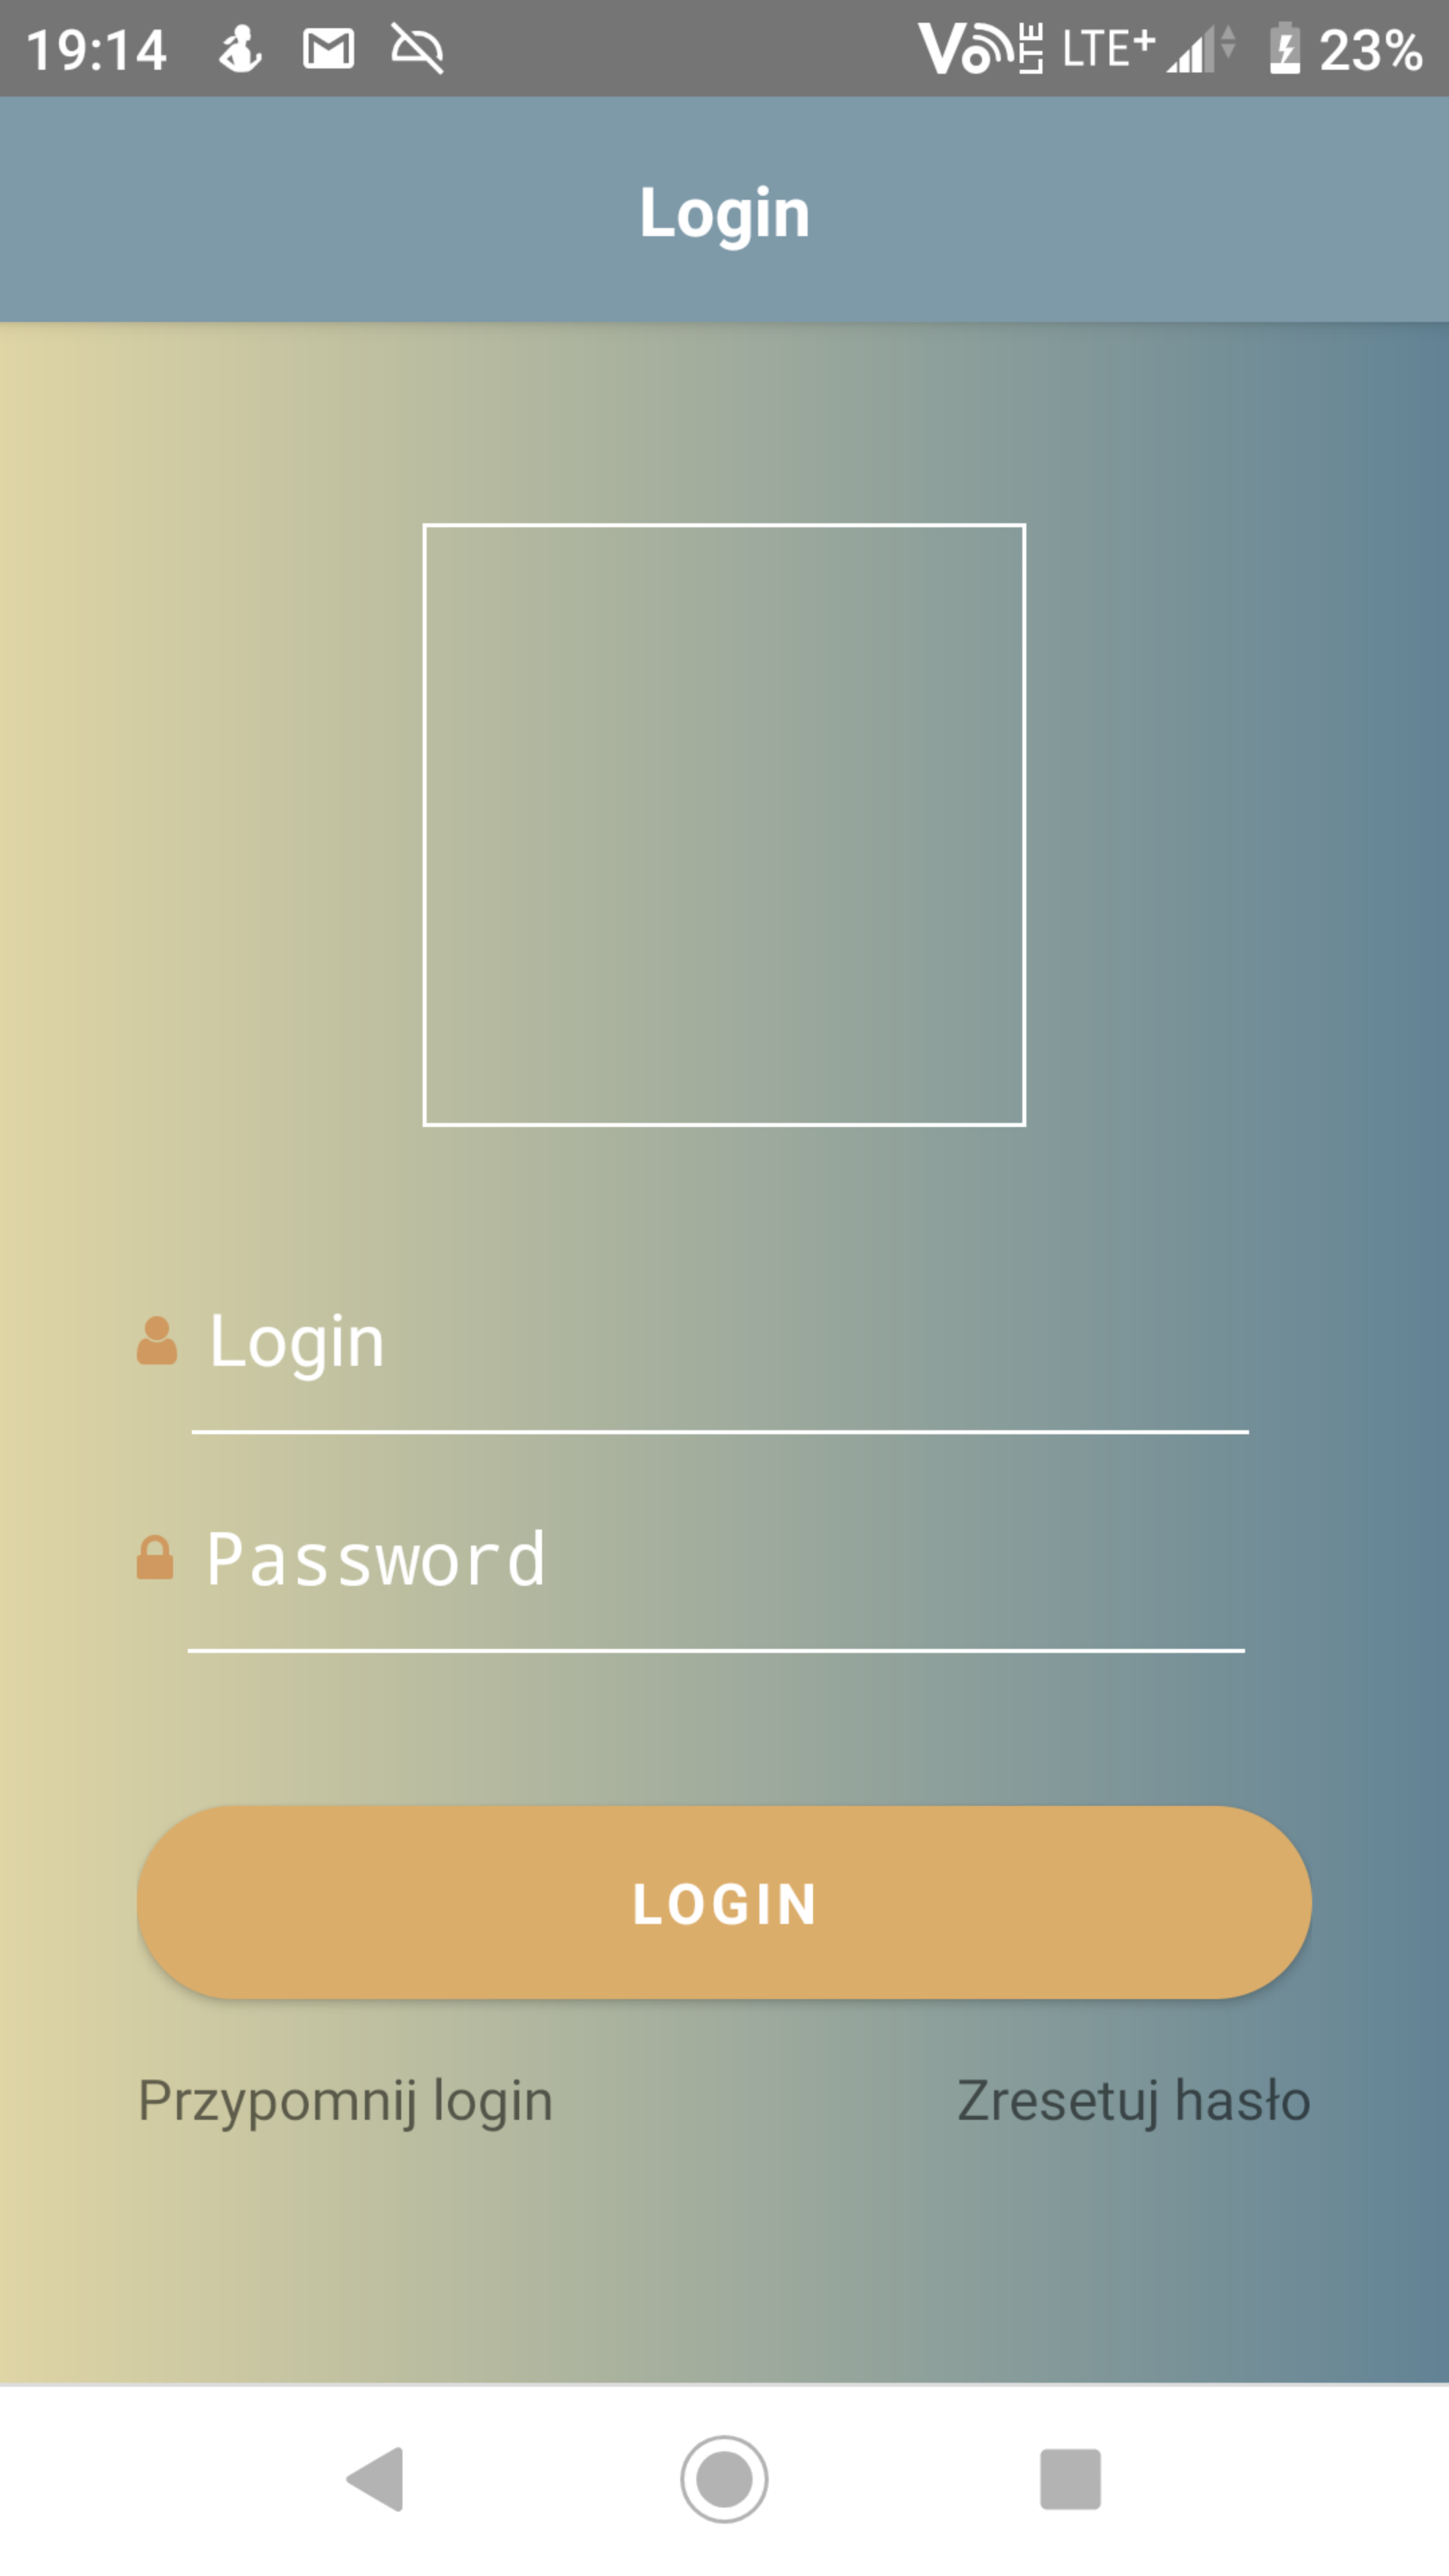
\includegraphics[scale=0.15]{images/mobileLogin.png}
\caption{Przykładowy wygląd strony logowania w aplikacji mobilnej}
\end{figure}

\section{Interfejsy zewnętrzne}
\subsection{SMTP}
Protokół SMTP jest używany do wysyłania wiadomości email z systemu. Jest to stary, prosty i sprawdzony protokół oparty na komunikacji TCP, implementowany przez większość (o ile nie wszystkich) dostawców poczty internetowej.
\subsection{Integracja DotPay}
Potrzebne będzie zaimplementowanie protokołów i procesu dokonywania płatności dostarczane przez DotPay. Po wstępnej analizie proces ten jest podobny do dobrze znanego procesu OAuth2. System DotPay nie implementuje żadnego ogólnodostępnego standardu, jednak ich standard jest dobrze udokumentowany i z przykładami. \cite{dotpay}

\section{Wybór technologii}
\subsection{Języki programowania}
Do implementacji systemu zostały wykorzystane następujące języki programowania: 
\begin{itemize}
    \item C\# (warstwa logiki biznesowej, API, testy logiki i API)
    \item TypeScript/JavaScript (aplikacja webowa i mobilna oraz ich testy)
    \item SQL (język do komunikowania się z bazą danych, głównie autogenerowany przez Entity Framework)
    \item Python (skrypt wczytujący karty egzaminacyjne)
\end{itemize}

\subsection{Użyte biblioteki}
\subsubsection{Aplikacja mobilna}
Głównym frameworkiem pozwalającym na budowę systemu na telefony z systemem Android jest NativeScript \cite{ns}. W aplikacji mobilnej jest wykorzystywany jego plugin nazwany NativeScript-Vue, pozwalający na pisanie aplikacji w sposób bardzo podobny do tego, jakbyśmy projektowali aplikację webową za pomocą frameworka Vue.js \cite{vue}.
\\
Innymi bibliotekami użytymi w aplikacji mobilnej są: 
\begin{itemize}
    \item axios - do wykonywania zapytań HTTP \cite{axios}
    \item nativescript-background-http - do ściągania zdjęć z serwera \cite{ns-http}
    \item nativescript-camera - do robienia zdjęć \cite{ns-cam}
    \item nativescript-feedback - wyświetlanie powiadomień w aplikacji \cite{ns-feed}
    \item nativescript-imagepicker - do wyboru zdjęcia z galerii \cite{ns-img}
    \item nativescript-local-notifications - pokazywanie powiadomień o przychodzących wiadomościach \cite{ns-notif}
    \item nativescript-ui-sidedrawer - panel boczny aplikacji \cite{ns-drw}
    \item nativescript-urlhandler - wykrywanie powrotu do aplikacji mobilnej z płatności \cite{ns-uha}
    \item rxjs - śledzenie zmian komponentów po zalogowaniu \cite{rxjs}
    \item vue-class-component, vue-property-decorator - poprawna obsługa TypeScriptu dla NativeScripta \cite{vue-cc} \cite{vue-pd}
    \item vuex - przechowywanie informacji zalogowanego użytkownika w trakcie działania aplikacji \cite{vuex}
\end{itemize}
\subsubsection{Aplikacja webowa}
Analogicznie głównym frameworkiem użytym w aplikacji webowej jest Vue.js.
Dodatkowe biblioteki to:
\begin{itemize}
\item axios - komunikacja sieciowa,
\item file-saver - zapisanie pliku,
\item material-design-icons-iconfont -ikony,
\item vuetify - wspomniana wcześnie paczka z komponentami widoku,
\item vuetify-datetime-picker
\item oraz inne zaimportowane poprzez zależności lub udział w procesie ładowania: inversify, node-gyp, ajv, popper.js, ts-loader
\end{itemize}

Biblioteki wymagane podczas kompilacji i rozwoju aplikacji: aspnet-webpack, awesome-typescript-loader, bootstrap, copy-webpack-plugin, css-loader, deepmerge, eslint, eslint-config-standard, eslint-friendly-formatter, eslint-loader, eslint-plugin-html, eslint-plugin-promise, eslint-plugin-standard, extract-text-webpack-plugin, fibers, file-loader, jquery, sass, sass-loader, style-loader, typescript, url-loader, vue-loader, vue-property-decorator, vue-style-loader, vue-template-compiler, webpack, webpack-bundle-analyzer, webpack-cli, webpack-dev-middleware, webpack-hot-middleware, webpack-merge.

\subsubsection{API i logika}
Do zaimplementowania logiki systemu oraz API będą wykorzystane następujące frameworki:
\begin{itemize}
    \item ASP.NET Core - biblioteka odpowiadająca za działanie serwera,
    \item Pomelo.EntityFrameworkCore.MySQL - do mapowania obiektów z bazy danych na klasy w logice i na odwrót,
    \item FluentValidation - silnie typowane walidacje dla modeli,
    \item IdentityServer4 - OpenID Connect i OAuth 2.0 framework dla ASP.NET Core,
    \item PdfSharpCore, QRCoder, ZXing - biblioteki służące do generowania i sczytywania dokumentów,
    \item oraz liczne pomocnicze biblioteki z środowiska .NET Core.
\end{itemize}

\subsubsection{Testy}
W testach będzie użyte kilka bibliotek: 
\begin{itemize}
    \item NUnit - framework do testów jednostkowych
    \item Moq - framework do tworzenia atrap obiektów do testów
\end{itemize}

\subsection{Platformy}
Środowiskiem wykonawczym aplikacji jest Docker, który jest wspierany na wszystkich popularnych platformach.

\subsection{System operacyjny}
\subsubsection{Aplikacja webowa}
Z aplikacji webowej możemy korzystać na każdym systemie operacyjnym, który posiada przeglądarkę zgodną z wymaganiami niefunkcjonalnymi aplikacji. 
\subsubsection{Aplikacja mobilna}
Aplikacja mobilna zadziała na telefonach z systemem Android w wersji większej bądź równej wersji 4.1 (Jelly Bean).
\subsubsection{API}
Api jest napisane na platformę .NET Core która jest dostępna na wszystkich głównych systemach operacyjnych: Windows, Linux i macOS.\cite{dotnetcore} Należy jednak pamiętać, że maszyna musi mieć dużą moc obliczeniową oraz wysoką prędkość łącza internetowego, najlepiej łącze symetryczne.
\subsubsection{Baza danych}
Serwer MySQL jest dostępny wszystkich głównych systemach operacyjnych: Windows, Linux, macOS i inne.\cite{mysqlwiki} Należy jednak pamiętać, że maszyna musi mieć dużą moc obliczeniową oraz wysoką prędkość łącza internetowego, najlepiej łącze symetryczne. Powinna również być w tej samej sieci co API - VPN lub LAN.
\section{Historia dokumentu}

\begin{tabularx}{\linewidth}{|X|l|l|X|}
    \hline
    Autor & Data & Wersja & Wprowadzone zmiany \\
    \hline
    Andrzej Westfalewicz, Filip Zyskowski & 04.11.2019 & v0.1 & Pierwsza wersja dokumentu \\
    \hline
    Andrzej Westfalewicz, Filip Zyskowski & 05.11.2019 & v0.1 & Poprawki pierwszej wersji dokumentu \\
    \hline
\end{tabularx}

\begin{thebibliography}{99}
\bibitem{ns} Strona frameworka NativeScript \href{https://www.nativescript.org/}{\underline{https://www.nativescript.org/}}

\bibitem{vue} Strona frameworka Vue.js \href{https://vuejs.org/}{\underline{https://vuejs.org/}}

\bibitem{axios} axios \href{https://github.com/axios/axios}{\underline{https://github.com/axios/axios}}
\bibitem{ns-http} nativescript-background-http \href{https://github.com/NativeScript/nativescript-background-http}{\underline{https://github.com/NativeScript/nativescript-background-http}}
\bibitem{ns-cam} nativescript-camera \href{https://github.com/NativeScript/nativescript-camera}{\underline{https://github.com/NativeScript/nativescript-camera}}
\bibitem{ns-feed} nativescript-feedback \href{https://github.com/EddyVerbruggen/nativescript-feedback}{\underline{https://github.com/EddyVerbruggen/nativescript-feedback}}
\bibitem{ns-img} nativescript-imagepicker \href{https://github.com/NativeScript/nativescript-imagepicker}{\underline{https://github.com/NativeScript/nativescript-imagepicker}}
\bibitem{ns-notif} nativescript-local-notifications \href{https://github.com/eddyverbruggen/nativescript-local-notifications}{https://github.com/eddyverbruggen/nativescript-local-notifications}
\bibitem{ns-drw} nativescript-ui-sidedrawer \href{https://www.npmjs.com/package/nativescript-ui-sidedrawer}{\underline{https://www.npmjs.com/package/nativescript-ui-sidedrawer}}
\bibitem{ns-uha} nativescript-urlhandler \href{https://github.com/hypery2k/nativescript-urlhandler}{\underline{https://github.com/hypery2k/nativescript-urlhandler}}
\bibitem{rxjs} rxjs \href{https://github.com/ReactiveX/RxJS}{\underline{https://github.com/ReactiveX/RxJS}}
\bibitem{vue-cc} vue-class-component \href{https://github.com/vuejs/vue-class-component}{\underline{https://github.com/vuejs/vue-class-component}}
\bibitem{vue-pd} vue-property-decorator \href{https://github.com/kaorun343/vue-property-decorator}{\underline{https://github.com/kaorun343/vue-property-decorator}}
\bibitem{vuex} vuex \href{https://github.com/vuejs/vuex}{\underline{https://github.com/vuejs/vuex}}

\bibitem{dotnetcore} Strona główna oprogramowania .NET Core \href{https://dotnet.microsoft.com/download}{\underline{https://dotnet.microsoft.com/download}}

\bibitem{mysqlwiki} Wikipedia: MySQL \href{https://pl.wikipedia.org/wiki/MySQL}{\underline{https://pl.wikipedia.org/wiki/MySQL}}

\bibitem{dotpay} Dotpay - Technical manual for payments implementation
\href{https://www.dotpay.pl/developer/doc/api_payment/en/}{\underline{https://www.dotpay.pl/developer/doc/api\_payment/en/}}
\end{thebibliography}

\end{document}
